\documentclass[12pt]{article}
\usepackage{graphicx}
\usepackage{wrapfig}
\usepackage{amsmath}
\usepackage{fancyhdr}
\usepackage{hyperref}
\usepackage[margin=1.0in]{geometry}
\raggedbottom
\frenchspacing
\newcommand{\HRule}{\rule{\linewidth}{0.5mm}}
\begin{document}

\pagestyle{fancy}
\lhead{8-Puzzle Search Algorithms}
\chead{spn1}
\rhead{Spencer Newton}
\cfoot{\thepage}

\begin{titlepage}
\begin{center}
\HRule \\[0.2cm]
{\huge Introduction to Intelligent Systems \\[0.2cm] }
{\Large Informed and Uninformed Search for 8-Puzzle Solutions \\[0.2cm]}
\HRule \\[0.4cm]
{\large Spencer Newton \\[0.2cm]}
{\large November / December 2014 \\[0.5cm]}
\begin{figure}[h]
	\centering{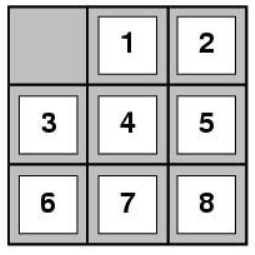
\includegraphics[scale = 0.8]{Images/8puzzlepiccomplete.png}}
	\caption{An example of the 8-Puzzle grid}
\end{figure}
\end{center}
\end{titlepage}


\tableofcontents

\newpage

%==================================================================================================
%								Introduction
%==================================================================================================
\section{Introduction}
Searching is a common task that is given to computers, and so it is important to invent algorithms that can do this quickly and efficiently. In addition to searching through known lists and directories, solutions to problems and puzzles can be found using computers in a similar way. Effort has been put into researching artificially intelligent ways of solving such problems in different ways, such as by informing the algorithm of the state of the search in order to guide its progress. This report details an experiment to analyse the performance of four search algorithms, two of which are informed of their search progress, and two which are not.

These algorithms were applied to a puzzle called the N-Puzzle. This puzzle consists of a 3 by 3 grid of slots, filled with 8 tiles numbered 1 through 8, with one empty slot. The grid is initially randomly arranged with tiles, and the goal is to get the tiles in a specific order (Figure 1), however tiles can only be moved into an adjacent slot if it is empty. This causes the puzzle to be complex and difficult for a human to solve, and therefore a problem best left for computers to solve.

The following report is split into 3 sections. The first, Program Design, details the architecture and implementation of the program, as well as discussions and justifications of the choices made. The second, Experimentation, details the experiments conducted to test the program and algorithms. The third and final section, Results \& Discussion, presents the outcome of the experiments and discusses the performance of each algorithm with respect to the quality of the program and the properties of the algorithms.

%==================================================================================================
%								Design
%==================================================================================================
\section{Program Design}
The first task was to design and code the program. There are many examples of N-puzzle programs on the internet as it is a common problem to demonstrate with, however I chose to look for other ways people have implemented search algorithms. I drew inspiration from the path-finding examples for this module as a place to start my design. For these examples, various search algorithms were implemented to search through a large 2D grid of tiles for a path between two points on the grid. In this case, the search space consisted of a 2D array of tiles that could be moved to. For the 8-puzzle, the search space consists of all the possible states that can exist in the puzzle (9!), whereby adjacent states are considered to be 1 legal move between each other.

\subsection{Design}
The program design is as follows and can be seen in UML format in Figure \ref{fig:umldiag}. A state of the grid is encapsulated into the PuzzleGrid class. This class contains a 2D array of integers, representing the state of the grid, as well as other attributes such as the size of the grid and the position of the empty space. The grid is capable of being loaded from a file in a specific format, or copied from another PuzzleGrid object. Finally, there is a function that allows the empty slot in the grid to be moved around in a legal manner.

Other information regarding the grids, such as their parents / children during the search need to be known, but rather than putting this in the PuzzleGrid class a new class was created called PuzzleNode. This represents the state of a PuzzleGrid in search space and includes a list of it's children and parent. A component of it is a heuristic object, which contains the heuristic value of that node. PuzzleNodes are created with PuzzleGrids and modified by the search algorithms to find the solution to the puzzle.

At this point, search algorithms and heuristics have been mentioned, however there are various different implementations in the program, and so each one has their own interface. The interface that represents a search algorithm is called SolutionFinder. Classes that implement this need to override two functions: findSolution() and printSearchData(). The former must return an ArrayList of PuzzleNodes representing the path from start to end (or null for no path), and the latter must print out data regarding the search (ie Nodes expanded, time taken). The interface that represents a heuristic is called Heuristic. Classes that implement this need to override two functions: calculateHeuristic() and getHeuristicValue(). The first is used to calculate the heuristic using the current state of the search and the goal state, while the latter simply returns the heuristic value that should have been calculated.

There is one implementation of the SolutionFinder interface for each search algorithm tested, which are Depth-first search, Breadth-first search, Greedy Best-first search, and A* search. Each sub-class implements the search algorithm in the inherited function findSolution(). For these three algorithms, three different heuristics were used, all of which implemented the Heuristic interface. The GreedyHeuristic sub-class takes into account the estimated remaining path cost to the goal and the AStarHeuristic sub-class takes into account the total path cost so far as well as the estimated remaining path cost. The third heuristic, EmptyHeuristic, is for uninformed search methods whereby no heuristic is used; this simply returns a constant value.

This is all run through the Solve class which contains the entry point to the program and the execution routine. The main method requires three arguments to function, which are two filenames containing the initial and end states of the puzzle, and a character code indicating the search algorithm to be used. Assuming that these arguments are valid, two PuzzleGrids are instantiated to represent the start and end states from the file arguments, the correct SolutionFinder sub-class is initialised, and then the search is started using the findSolution() method. Assuming the solution path is found, it is printed out to console along with data regarding the search and input parameters.

\begin{figure}[!h]
	\begin{center}
		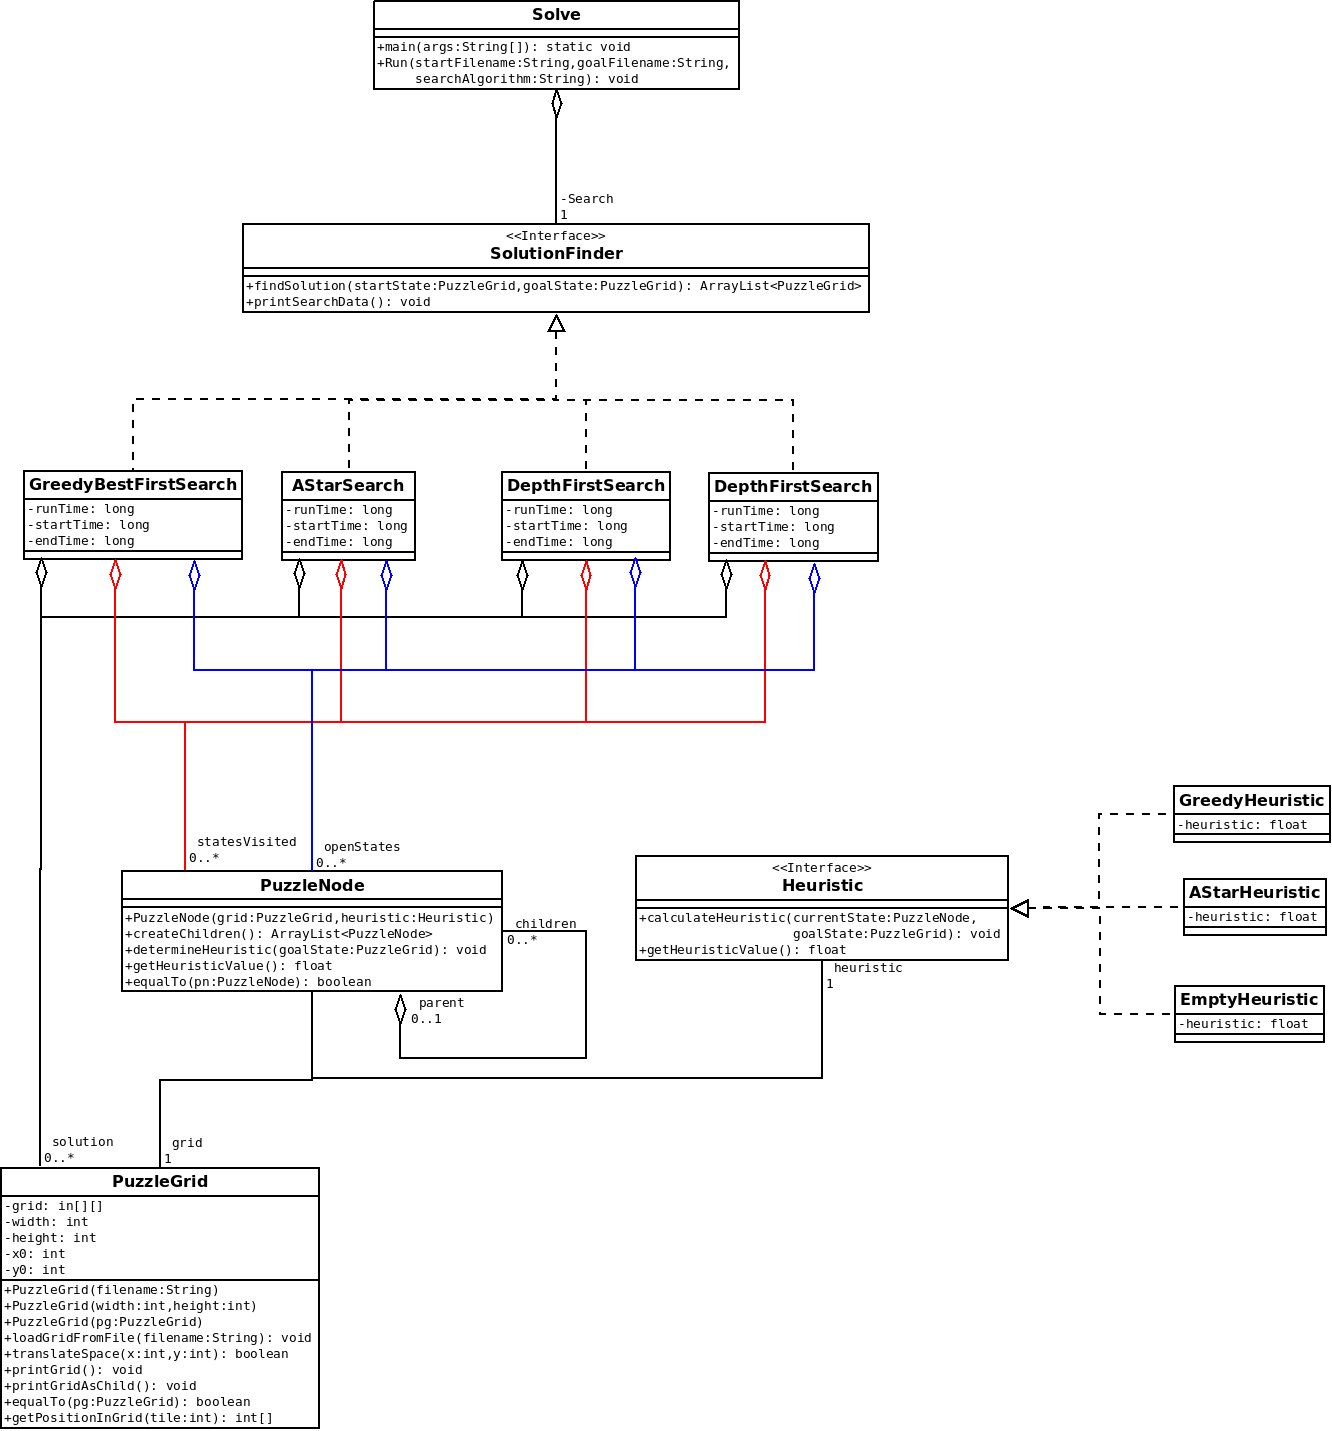
\includegraphics[scale=0.3]{Images/UML_diagram.png}
		\label{fig:umldiag}
		\caption{A UML Diagram showing the class structure of the program.}
	\end{center}
\end{figure}

\subsection{Implementation}
The implementation of this design went smoothly. Apart from gathering ideas and inspiration from other sources, the design was mostly thought about during coding. The main ideas that I thought were important when I started were as so:
\begin{itemize}
	\item A way is needed of representing the state of the grid and data relating to the state during a search.
	\item The design should be object oriented to help with the implementation of multiple similar features.
	\item The search and heuristic classes should be implemented in a modular way so that they can be easily interchanged.
\end{itemize}
The first idea was realised as the PuzzleGrid and PuzzleNode classes. Initially, the data relating to the search in PuzzleNode (such as children / parents) was going to be a part of PuzzleGrid, but I wanted to encapsulate the two different kinds of data into two separate classes. The set of data relating to the search was put in one class, while the set of data relating to the grid should be in another.

When it came to implement the search algorithms, a common interface (SolutionFinder) was used to allow for simple interchanging. I found that most of the code in the algorithms was very similar; most of the change came from the heuristics and the data structures used to represent the search space. This result in some code copy / pasting between classes (written by myself), which could have been avoided by making the SolutionFinder an abstract class instead of an interface, and implementing the minor differences into sub-classes. The main variations were that DFS used a stack to store open states instead of a LinkedList (used like a Queue). Due to the way child nodes were generated (which was in the order of moving the empty tile up, left, right, then down), the children were added to the stack in reverse order compared to the other algorithms. The remaining differences were in the heuristics, which were encapsulated into separate classes.

At some points during the algorithms, it is required that the lists of open states and states already visited be searched to see if they contain a particular grid state. For this, I attempted to use the contains() method for the lists, however this checks whether the objects are directly equal by hash code. I required that the list check whether they were equal by contents (the grid state), so I wrote code to manually check the grid arrays between each element in the lists and the state under scrutiny. In retrospect I could have rewritten the equals() or hashcode() method so that the contains() method worked correctly, which could have made the algorithms run quicker.

I initially started working on the uninformed search methods (Breadth-first and Depth-first) and thus did not immediately worry about heuristics. Eventually I started to implement informed search algorithms and so I refactored my code to include heuristics. This was a simple process, as I modularised the heuristics into different classes. When the first PuzzleNode is created, it is constructed with one of three implementations of the Heuristic interface, depending on what algorithm is being used. From then on, when child nodes of that state are created, reflection is used to create new heuristic objects of the same type. The value of a heuristic attached to a PuzzleNode is obtained by calling the function calculateHeuristic() and getHeuristicValue().

Once the heuristic had been calculated for each node, it would then be added to a list of open states. This required (for the informed methods) that this list be sorted in order of ascending heuristic value. For this, I manually compared the heuristic values of each element to find where the subject node should be placed. In retrospect, I could have implemented a built-in interface, such as Comparator, and let the list sort itself. Since I did not do this, I did not have to use an ordered data structure such as a priority queue.

In addition to all of this, data was collected in the SolutionFinder sub-classes in order to analyse the perform of each algorithm. This data was printed out into the console upon completion of the searches. The following sections detail the experiments that were conducted on the algorithms and the results that were obtained.

%==================================================================================================
%								Experimentation
%==================================================================================================
\section{Experimentation}
In order to investigate the performance of each algorithm, test cases were created. These tests involved specifying the start and goal states of the puzzle and feeding them into the program to solve. The test cases are split into two sets and can be seen in Figure \ref{fig:testcases}. Test Case Set 1 is the set of default tests provided with the assignment plus one additional start state, chosen randomly. Test Case Set 2 is a set of alternative states discovered on the internet \cite{web:moretests}. These were chosen as they had a different goal state and could be used to test whether the program functions in a slightly different variation of the puzzle. 

\begin{wrapfigure}{l}{0.4\textwidth}
	\begin{center}
		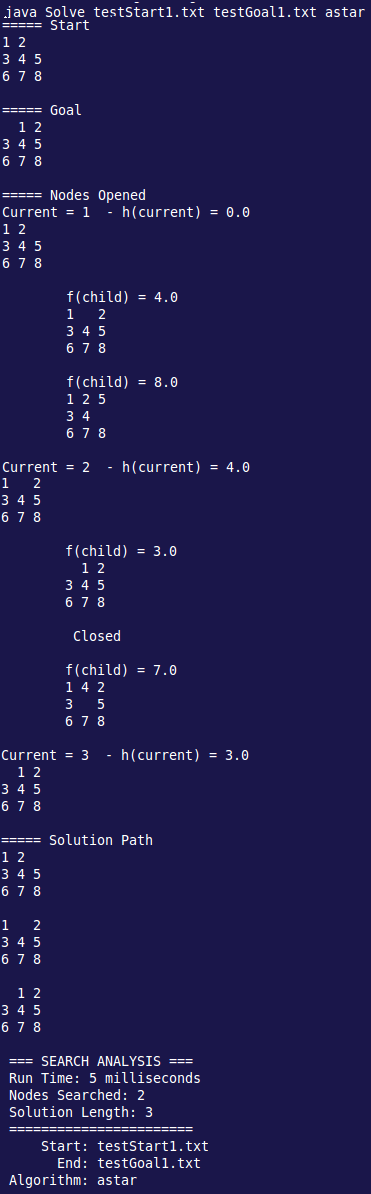
\includegraphics[scale=0.4]{Images/example_output.png}
		\label{fig:examplerun}
		\caption{An image showing and example of the output of the program.}
		\vspace{-60pt}
	\end{center}
\end{wrapfigure}

The grid data in Figure \ref{fig:testcases} was supplied as input to the program via '.txt' files in a specific format - adjacent tiles on the same row separated by a comma, rows separated by a new line. Test Case Set 1 was contained in files named testGoal1.txt and testStart1/2/3/4.txt. Test Case Set 2 was contained in files named tg1.txt and ts1/2/3/4.txt. These files are fed as arguments into the program which attempts to find a solution path between the two states using whatever algorithm is specified in the third argument. During the execution of the program, it will print out the grid states that it searches and opens. Once it has finished it will print out the final solution path it has found. An example execution can be seen in Figure \ref{fig:examplerun}.

The tests were run directly from the command line on an Intel Core i7 Mobile CPU running Ubuntu 14.04 TLS. Each test was run on it's own with minimal CPU load on the computer to avoid external influence on the run times. Once each test was finished, the data gathered was recorded and can be seen in Tables \ref{tbl:DataSet1} and \ref{tbl:DataSet2}, one for each set of tests.


%==================================================================================================W
%								Results & Discussion
%==================================================================================================
\section{Results \& Discussion}

The results vary significantly between each algorithm. For each method, the results will be discussed, and then will be compared with each other. The algorithms can be separated into two categories: Informed and Uninformed searches. The algorithms that are not aware of the current state of the search are referred to as uninformed (Breadth-first and Depth-first), while the ones that are given information about the state of the search are known as informed (Greedy Best-first and A*). It is important to compare the two because in certain cases the informedness of the algorithm has a large effect on the outcome of the search.

It should be noted that because of the way the algorithms were programmed, the run-time gets exponentially longer the more difficult the problem is. This is because it will iterate through every state in the list of open and visited states every time it checks a new node. Therefore as more nodes are added to these lists, the longer the algorithm will take to check each new node. Thus the run-times for long searches may be over exaggerated.

\begin{figure}[h]
	\begin{center}
		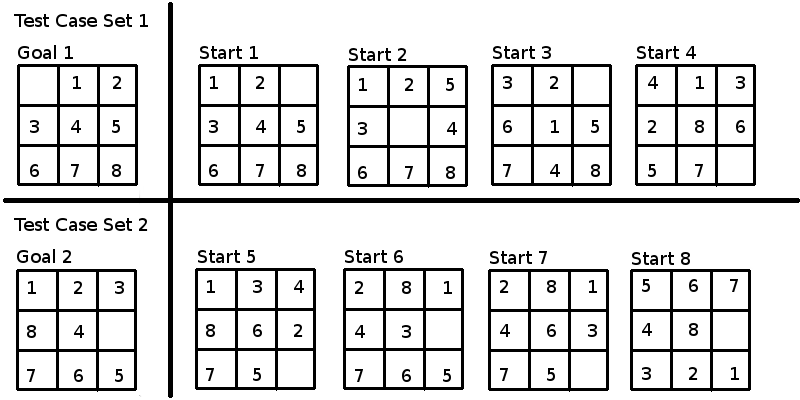
\includegraphics[scale=0.4]{Images/test_grids.png}
		\label{fig:testcases}
		\caption{An illustration showing the start and goal states used during the testing of the algorithms.}
	\end{center}
\end{figure}

\subsection{Uninformed Searches}
The uninformed search algorithms were Breadth-first (BFS) and Depth-first Search (DFS), and the results for Test Case Set 1 can be seen in Table \ref{tbl:DataSet1}. For the default cases in Test Case Set 1, both algorithms performed similarly, but there were some key differences in their outcomes. Most notable is that they both came out with different solutions, with BFS always coming out with the shortest and most optimals. This is because BFS always searches the shallowest portions of the search tree first and all the step costs are identical. Therefore, the first solution that it comes across will be the quickest one. DFS searches deep paths into the search tree first. This may result in non-optimal solutions and means it will search a lot more nodes before finding one. 



\begin{table}[h]
\centering
 	\begin{tabular}{l r r r}
   		Algorithm &     Time & Nodes Explored & Solution Length \\
   			\hline
   			Start 1 - Goal 1 \\
   			\hline
   		bfs & 2ms & 3 & 3 \\
   		dfs & 1ms & 2 & 3 \\
   		gbfs & 2ms & 2 & 3 \\
   		astar & 2ms & 2 & 3 \\
   		
   			\hline
   			Start 2 - Goal 1 \\
   			\hline
   		bfs & 23ms & 29 & 5 \\
   		dfs & 49ms & 62 & 59 \\
   		gbfs & 7ms & 7 & 5 \\
   		astar & 8ms & 7 & 5 \\	
   				
   			\hline
   			Start 3 - Goal 1 \\
   			\hline
   		bfs & 52ms & 67 & 7 \\
   		dfs & 92ms & 151 & 141 \\
   		gbfs & 9ms & 9 & 7 \\
   		astar & 9ms & 9 & 7 \\
   		
   			\hline
   			Start 4 - Goal 1 \\
   			\hline
   		bfs & 4725785ms & 178993 & 29 \\
   		dfs & 737561ms & 50520 & 44401 \\
   		gbfs & 101ms & 163 & 45 \\
   		astar & 38683ms & 8289 & 29 \\   		
  	\end{tabular}
  	
  	\caption{A table showing the results of running the program through case set 1.}
  	\label{tbl:DataSet1}
\end{table}

As the test cases get more complex this disadvantage of DFS becomes more apparent, as the test with the randomly chosen start (Start 4 - Goal 1) finds a solution with a length of 44401. It did find this solution in less time and by exploring fewer nodes than BFS however, but the solution length is too impractical. The reason why it found a solution faster is because the quickest path is relatively deep into the search tree, causing BFS to search much slower. Despite the longer time and larger search space it took to solve this test case, BFS still came out with an optimal solution. 
 
For most of Test Case Set 1, BFS performed better than DFS. For the final test (Start 4 - Goal 1) however, DFS performed better than BFS when it came to run-time and number of nodes searched. This seems odd, however it is due to the fact that nodes are searched in whatever order they are added to the queue or stack. Informed methods will add nodes to a priority queue based on some heuristic value unique to the algorithm. Therefore, for these uninformed search algorithms, their performance relies heavily on the implementation. In this case, it is whatever order the child nodes are added to the list of open states.

To tests the effect of the implementation of each algorithm, Test Case Set 1 was run again, except the child nodes were added in reverse order - in the order of having moved to empty square down, then right, then left, then up. The results can be seen in Table \ref{tbl:DataSet1alt}, and make the problem much more noticeable. Compared to the first set of results, DFS performs \emph{significantly} worse. Where previously it had mostly resulted in relatively short and simple solutions, reversing the order caused it to search almost the entire tree to try to find extremely long solutions. This is because the maximum path length in state space is very large for this puzzle, which results in a large time and space complexity. For BFS, reversing the order did cause a slight change in the performance, however due to how the algorithm works these solutions were only slightly different to the first results. Despite the changes in run-time and nodes searched for BFS, it still provided optimal solutions for all of the tests, regardless of the order nodes were searched.

Finally, Test Case Set 2 was fed into the program. This had a set of more complex puzzle, and the results of the algorithms reflect that. BFS consistently found optimal solutions after a moderate period of time. DFS on the other hand struggled to find solutions quickly and ended up taking an extremely long time to find very inefficient solutions. Only when the solution was deep enough into the search tree for BFS to take a long time did DFS out-perform it in terms of time and space complexity.

\begin{table}[h]
\centering
 	\begin{tabular}{l r r r}
   		Algorithm &     Time & Nodes Explored & Solution Length \\
   			\hline
   			Start 5 - Goal 2 \\
   			\hline
   		bfs & 99ms & 140 & 8 \\
   		dfs & 8022517ms & 180644 & 890 \\
   		gbfs & 11ms & 8 & 8 \\
   		astar & 8ms & 8 & 8 \\
   		
   			\hline
   			Start 6 - Goal 2 \\
   			\hline
   		bfs & 436ms & 1613 & 13 \\
   		dfs & 7039145ms & 145402 & 36137 \\
   		gbfs & 77ms & 111 & 19 \\
   		astar & 53ms & 65 & 13 \\	
   				
   			\hline
   			Start 7 - Goal 2 \\
   			\hline
   		bfs & 847ms & 2551 & 14 \\
   		dfs & 4104757ms & 83342 & 67384 \\
   		gbfs & 79ms & 114 & 20 \\
   		astar & 51ms & 66 & 14 \\
   		
   			\hline
   			Start 8 - Goal 2 \\
   			\hline
   		bfs & 7937948ms & 181378 & 31 \\
   		dfs & 3900566ms & 79883 & 65673 \\
   		gbfs & 145ms & 285 & 71 \\
   		astar & 11618ms & 5334 & 31 \\   		
  	\end{tabular}
  	
  	\caption{A table showing the results of running the program through case set 2.}
  	\label{tbl:DataSet2}
\end{table}

\subsection{Informed Searches}
The informed search algorithms were Greedy Best-first Search (GBFS) and A* Search (A*), which both make use of heuristics to sort child nodes as they are created in the tree. GBFS sorts them in order of estimated remaining path cost, while A* sorts them in order of estimated remaining path cost plus total path cost so far. The algorithms worked in a similar fashion to the uninformed methods, but the addition of the heuristics caused the results to improve significantly.

In Test Case Set 1, the two algorithms performed almost identically for all the tests, coming out with very short solutions in relatively small times and spaces. Disparities arose when the puzzle became complex (Start 4 to Goal 1). In this case, GBFS found a solution the fastest and by opening fewer nodes, however the solution was slightly longer than A*. This is because the Greedy heuristic is more concerned about finding a solution quickly, while the A* heuristic tries to find the solution quickly while also taking into account the path cost. In other words, A* is more \emph{informed} than GBFS. Also, when the solution is relatively deep into the search tree, A* is more likely to explore more paths, and thus take longer, as it adds more nodes to the frontier.

Both performed significantly better than the uninformed methods in the complex test case. A* did take a relatively long time to find a solution compared to GBFS, however it always resulted in the most optimal solution due to the fact that it always underestimates the estimated remaining path cost. In Test Case Set 2, disparities arose once more for the most complex problem (Start 8 to Goal 2), however differences can also be noticed in the simpler problems (although more complex than Test Case Set 1). In these cases (Start 5/6/7 to Goal 2), A* outperformed GBFS in both time and space while also finding more optimal solutions. This is most likely due to the slightly increased complexity while still having a shallow optimal solution. 

\begin{table}[h]
\centering
 	\begin{tabular}{l r r r}
   		Algorithm &     Time & Nodes Explored & Solution Length \\
   			\hline
   			Start 1 - Goal 1 \\
   			\hline
   		bfs & 7ms & 6 & 3 \\
   		dfs & 8102423ms & 169022 & 13171 \\
   		
   			\hline
   			Start 2 - Goal 1 \\
   			\hline
   		bfs & 19ms & 28 & 5 \\
   		dfs & 7283780ms & 139063 & 41769 \\	
   				
   			\hline
   			Start 3 - Goal 1 \\
   			\hline
   		bfs & 49ms & 74 & 7 \\
   		dfs & 5976878ms & 111950 & 63915 \\
   		
   			\hline
   			Start 4 - Goal 1 \\
   			\hline
   		bfs & 8437074ms & 179855 & 29 \\
   		dfs & 8049936ms & 169026 & 13217 \\ 		
  	\end{tabular}
  	
  	\caption{A table showing the results of running the uninformed search algorithms through case set 1 when they search through nodes in reverse order (in the order of moving the empty tile down - right - left - up, instead of up - left - right - down).}
  	\label{tbl:DataSet1alt}
\end{table}

\section{Conclusion}
Each algorithm was able to find a solution to the different puzzle states with varying degrees of success. The uninformed searches were simple to implement and could provide adequate solutions for easy problems, but as the puzzles got more complex the algorithms became very inefficient. This is due to the fact that the search space of this problem is very large, and with no heuristic the uninformed methods searched unintelligently through it. For this type of problem, informed methods are more appropriate.

The informed searches performed much better due to the information gained about the search in their heuristics. Both heuristics were admissible because they never overestimated the path costs (estimated and total). They did this by estimating the solution using a relaxed version of the puzzle. The algorithms were slightly more complex to implement, but reliably provided efficient and usable solutions for difficult puzzles. 

The informed algorithms displayed a trade-off in run-time and optimality when searching \textbf{complex} puzzles. For GBFS, the solution is found much quicker than A*, but the path is longer. A* takes longer to look through the search space, but since it is admissible it always provides an optimal solution. Where time is not too much of an issue, A* would be more applicable. Where time is an issue but the optimality of the solution is not (to a degree), GBFS would be better.

\newpage
%==================================================================================================
%								Bibliography
%==================================================================================================
\bibliographystyle{plain}
\bibliography{8puzzle_refs}


\end{document}